%-------------------------------------------------------------------------------
% live_grid
%-------------------------------------------------------------------------------
%
% \file        live_grid.tex
% \library     Documents
% \author      Chris Ahlstrom
% \date        2015-11-01
% \update      2024-12-02
% \version     $Revision$
% \license     $XPC_GPL_LICENSE$
%
%     This document provides LaTeX documentation for Seq66.
%
%-------------------------------------------------------------------------------

\section{Live Grid / Main Window and Tabs}
\label{sec:live_grid}

   For our walk-through of the main window, the following figure
   shows it using blue labels for reference.

\begin{figure}[H]
   \centering 
   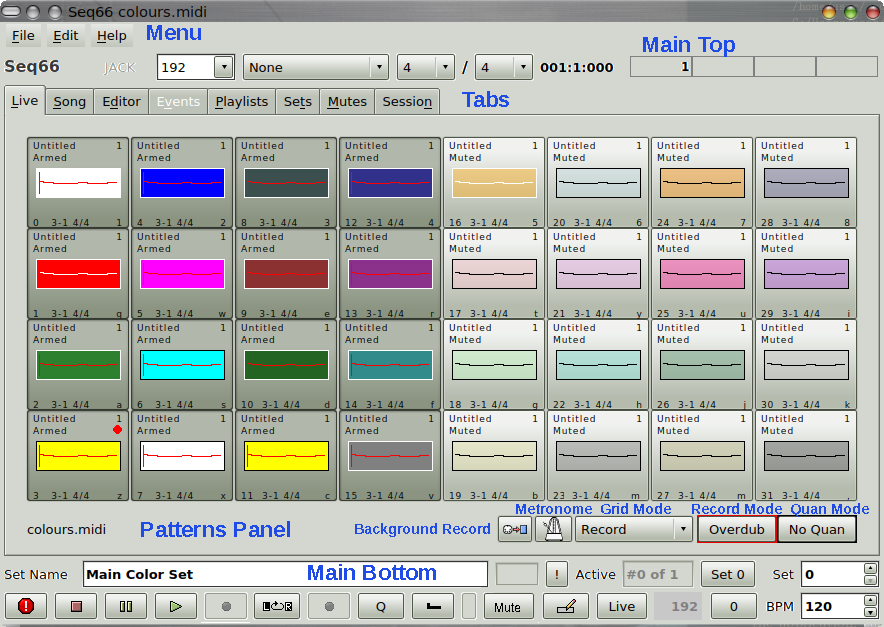
\includegraphics[scale=0.65]{main-window/main-window-annotated.png}
   \caption{Seq66 Main Screen, Annotated}
   \label{fig:main_screen_annotated}
\end{figure}

   The \textsl{Seq66} main window (i.e. the "Live Grid") appears as shown above.
   This figure has many differences from the \textsl{Seq24} main window,
   but the functionality is similar.
   \textsl{Seq66} allows resizing, and can
   be configured to start with its size scaled up or down.
   There is also a button near the top (not shown) that can
   hide the menu and the bottom panels, to allow reducing the
   size of the window event further.
   Its features, including the "look" of the application,
   can be configured via the 'rc', 'usr', 'ctrl', 'drums', 'playlist', 'mutes',
   and 'palette' configuration files, via command-line options, via
   desktop themes, and via Qt ('qss') style-sheets.
   We break the discussion into sections for the following
   groups shown in the figure above:

   \begin{itemize}
      \item \textbf{Tabs}
      \item \textbf{Main Top}
      \item \textbf{Main Bottom}
      \item \textbf{Menu}
   \end{itemize}

\subsection{Tabs}
\label{subsec:introduction_main_tabs}

   The following tabs are present in \textsl{Seq66}:

   \begin{itemize}
      \item \textbf{Live}
      \item \textbf{Song}
      \item \textbf{Editor}
      \item \textbf{Events}
      \item \textbf{Playlists}
      \item \textbf{Sets}
      \item \textbf{Mutes}
      \item \textbf{Session}
   \end{itemize}

   We present brief descriptions here and links to sections with more detail.
   All tabs are discussed in more detail, each in its own section.

\subsubsection{Tabs / Live}
\label{subsubsec:introduction_main_tabs_live}

   The \textbf{Live} tab is foremost in the application.
   It provides a grid of \textsl{patterns}
   (also called \textsl{slots}, \textsl{loops}, \textsl{tracks}, or
   \textsl{sequences}) that display recorded MIDI data, status information, and
   provide popup-menus for each pattern.
   The buttons can
   be colored via a palette, and the status is easy to see
   from the coloring of activated buttons and a label that says "Armed"
   versus "Muted".
   The buttons can be toggled by a keystroke, shown in the lower
   right corner of the button.
   Another name for the \textbf{Live} tab is the \textbf{Patterns Panel};
   it can be replicated in multiple external windows.
   See \sectionref{sec:patterns_panel}.

\subsubsection{Tabs / Song}
\label{subsubsec:introduction_main_tabs_song}

   The \textbf{Song Editor} combines all patterns
   into a complete tune with controlled repetitions of each pattern.
   It provides a way to lay out \textsl{triggers} for each pattern
   that control playback without musician interaction.
   The editing capabilities of the song editor are extensive, including
   dragging triggers, addition transposition to triggers, and more.
   See \sectionref{sec:song_editor}.

\subsubsection{Tabs / Editor}
\label{subsubsec:introduction_main_tabs_editor}

   The \textbf{Pattern Editor} allows for the recording and editing of
   notes and other MDII events.
   It can be shown in the \textbf{Editor} tab or in an
   external window.  When opened in the tab, the pattern editor is compressed
   vertically by reducing the height of the "data" area and removing some
   buttons.  Otherwise, the pattern editor works the same in the tab and in
   external windows.
   See \sectionref{sec:pattern_editor}.

\subsubsection{Tabs / Events}
\label{subsubsec:introduction_main_tabs_events}

   The \textbf{Event Editor} provides a way to see the details of events
   and to do some modifying of them.  It's meant for light usage; there are
   some less-used events that it cannot edit.
   It is especially useful in trouble-shooting a song.
   See \sectionref{sec:event_editor}.

\subsubsection{Tabs / Playlist}
\label{subsubsec:introduction_main_tabs_playlist}

   The \textbf{Playlist Editor} is meant for the creation of
   play-lists.  One can create multiple playlists with multiple songs in each
   playlist.  The selection of playlists and songs can be done via keystrokes
   or MIDI control.
   Note that editing of the playlists can also be done by directly editing a
   \texttt{.playlist} file.  See \sectionref{sec:playlist}.

\subsubsection{Tabs / Sets}
\label{subsubsec:introduction_main_tabs_sets}

   The \textbf{Sets Editor} allows one to see, edit, and rearrange the sets
   that a tune contains.  Sets are also referred to as "banks".
   A useful feature of sets is that they can selected and cause a major change
   in the patterns that are playing.
   See \sectionref{sec:setmaster}.

\subsubsection{Tabs / Mutes}
\label{subsubsec:introduction_main_tabs_mutes}

   Mute-groups provide a way to turn on and turn off multiple patterns at once
   via a keystroke or a MIDI control; the \textbf{Mutes Editor} also provides a
   way to use buttons to control the mute-group.
   Mute-groups can be saved in the
   \texttt{.mutes} file or in the tune itself.
   See \sectionref{sec:mutes_master}.

\subsubsection{Tabs / Session}
\label{subsubsec:introduction_main_tabs_session}

   The \textbf{Session} tab displays some aspects of the running setup of
   \textsl{Seq66}.  It displays the name of the session manager, if any, client
   IDs, etc.  It also has a button reload the whole session after configuration
   changes are made.

   Here, a session log file can also be specified.
   If defined, then all messages written to the terminal when \textsl{Seq66}
   is run from a terminal shell are instead redirected to this file.
   The default log file is \texttt{seq66.log} specified to use
   the "home" directory.
   This file can be cleared using the button to the right of it; however,
   messages will continue to be logged to this file until
   \textsl{Seq66} is completely exited and then manually restarted.

   In addition, text data for patterns can be viewed and edited here.
   Select the desired pattern, enter the desired text, and click the
   \textbf{Save Info} button.
   The song is now modified and can be saved.

   Also see \sectionref{sec:sessions}.

\subsection{Main Top Controls}
\label{subsec:introduction_main_top_controls}

   Here, we first discuss the top and bottom \textbf{Main} controls, as
   shown in the following collapsed figure:

\begin{figure}[H]
   \centering 
%  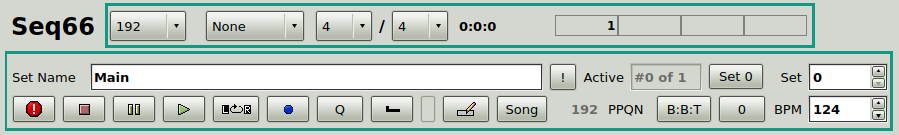
\includegraphics[scale=0.75]{main-window/main-window-controls.png}
   
\includegraphics[scale=0.75]{main-window/main-window-top.png}
   \caption{Main Window Top Controls}
   \label{fig:main_window_top_controls}
\end{figure}

   See the following section and
   \sectionref{subsec:introduction_main_bottom_controls}.
   The top panel of the Pattern window is simple, consisting of the
   name of the program and a few controls.
   The top main control items are, from left to right:

   \begin{itemize}
      \item \textbf{Seq66 Logo}
      \item \textbf{Show/Hide Button}
      \item \textbf{Engine Status}
      \item \textbf{PPQN Selection}
      \item \textbf{Buss Override for Play-set}
      \item \textbf{Global Beats Per Measure}
      \item \textbf{Global Beat Width}
      \item \textbf{BBT/HMS Time Display}
      \item \textbf{Beat Indicator Bar}
   \end{itemize}

   The status indicators that can appear to the right of the logo:

   \begin{itemize}
      \item \textbf{ALSA} appears if running using ALSA for MIDI.
      \item \textbf{JACK} appears if running using JACK for MIDI.
      \item \textbf{JACK Master} appears if running using JACK transport, as
         transport master.
         JACK transport can be used even if using ALSA for MIDI.
      \item \textbf{JACK Slave} appears if using JACK transport as
         transport slave.
      \item \textbf{Portmidi} appears if using the internal portmidi-derived
         MIDI engine.  This is currently always the case on \textsl{Windows}.
   \end{itemize}

\subsubsection{Show/Hide Button}
\label{subsubsec:introduction_show_hide_button}

   If present (it is a build option),
   this button at the left of the top bar
   allows the main menu and the bottom two
   rows of controls to be hidden.
   This measure can save a lot of space (e.g. in a \textsl{Raspberry Pi}
   setup.
   If your window manager (e.g. \textsl{Fluxbox})
   allows hiding the window decorations, the smallest useful size of the
   main window can be about 450 x 320 pixels.
   Of course, a good 'ctrl' automation file (e.g. for the LaunchPad)
   is necessary to control \textsl{Seq66} in this tiny setup;
   main menu hot-keys are not accessible with the main menu hidden.

\begin{figure}[H]
   \centering 
   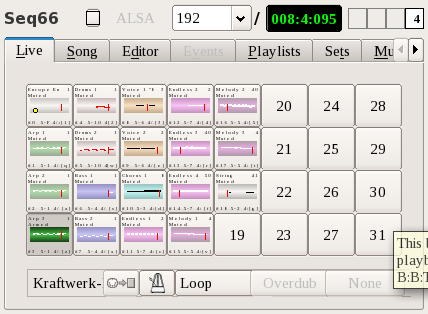
\includegraphics[scale=1.0]{main-window/main-window-tiny.png}
   \caption{Main Window Tiny (shown full size)}
   \label{fig:main_window_tiny}
\end{figure}

   Of course, most of the other tabs are not usable at this small size,
   the song editor menu, shortcut, and button aren't available,
   and the pattern editor still comes up big.
   Might be enough for live play?
   Perhaps we should add a 'usr' option for the "tiny" mode?
   And hide the rest of the tabs?  Switch some buttons around?

\subsubsection{PPQN Selection}
\label{subsubsec:introduction_ppqn_selection}

   This drop-down allows one to change the pulses-per-quarter-note (PPQN) of the
   loaded tune, and this change can then be saved, if desired, with the file.
   As with \textsl{Seq24}, the default PPQN is 192.
   \texttt{32, 48, 96, 120, 192, 240, 384, 768, 960, 1920, 2400, 3840,
   7680, 9600, and 19200}.
   The PPQN cannot be changed to to values not in this list, though.
%  Values, even weird ones, can be entered by typing them.
%  However, some values, such as 120, are not
%  displayed properly in the grids.
%  (Modify the file to use a supported value, if possible.)
   If a MIDI file is loaded, this modifies that file, rescaling all the
   pattern events and pattern triggers.
   Also see \sectionref{paragraph:menu_edit_preferences_play_options}.

\subsubsection{Buss Override for Play-set}
\label{subsubsec:introduction_sets_buss_override}

   This drop-down allows for overriding the buss (port) number used by all of
   the patterns in the current play-set.
   Unlike the \texttt{buss-override} setting in the 'usr' file
   (see \sectionref{subsubsec:usr_file_user_midi_settings}),
   this action causes a modification of the file (and a prompt to save at
   exit).

   \index{play-set}
   The \textsl{play-set} is the current set of patterns to be played.
   Normally, this set holds only the active patterns in the current
   play-screen.
   However, it can also be configured to include patterns from other sets.
   (See \sectionref{subsec:configuration_rc}.)

   The list of
   output busses is either the existing MIDI ports on the system, or,
   if port-mapping (see \sectionref{sec:port_mapping}) is active, the list
   of mapped output ports.
   Port-mapping is a useful way to redirect the set to a different output
   device; it can be used to provide a full set of virtual devices that any of
   the user's sequences can depend on.

   \index{--bus option}
   Another way to specify busses is the
   \texttt{-{}-buss n} command-line option.
   It causes \textsl{every} pattern in \textsl{every} set in the MIDI
   file to be directed to that buss number, and when a new
   sequence/pattern is created.  This option is only
   for convenience in testing.  Save the file, and it will
   have that buss number as part of each track's data, which makes the song
   file less portable, so be careful with both options.

\subsubsection{Global Beats Per Measure}
\label{subsubsec:introduction_global_beats_per_measure}

   This drop-down changes the global beats/measure for the song.
   Along with the beat-width setting, this set of values allows
   for a large number of different time signatures, even crazy ones.
   \textsl{Warning}: It modifies every pattern in the song, but is not
   otherwise saved in the configuration.
   Values: \texttt{1 to 16, 32}

\subsubsection{Global Beat Width}
\label{subsubsec:introduction_global_beat_width}

   This drop-down changes the global beat width (time-signature denominator)
   for the song.
   Along with the beats-per-measure setting, this set of values allows
   for a large number of different time signatures.
   \textsl{Warning}: It modifies every pattern in the song, but is not
   otherwise saved in the configuration.
   Values: \texttt{1 to 16, 32}

\subsubsection{BBT or HMS Time Display}
\label{subsubsec:introduction_time_display}

   This push-button shows the current time during playback. 
   It can be shown in BBT (bars:beats:ticks) or HMS (hours:minutes:seconds),
   which can be switched by clicking this button.
   (The \textbf{BBT/HMS} at the bottom of the window has been removed.)

\subsubsection{Beat Indicator}
\label{subsubsec:introduction_beat_indicator}

   The beat indicator is inspired by the \textsl{Kepler34} implementation.
   It shows the first beat in color, and the rest of the beats in the theme
   color.
   It does not adapt to changes in the time-signature until
   playback is stopped.

\subsection{Patterns Panel (Live Grid)}
\label{subsec:introduction_main_live_grid}

   In the center of the main window is the \textsl{patterns panel}, also 
   known as the \textsl{live grid}, where patterns/loops/tracks are shown
   and where they can be controlled.
   A MIDI file can be dragged-and-dropped onto the live grid in order
   to open it.
   Also shown in the patterns panel are a
   background-record button, metronome button, a
   grid-mode dropdown to control how the grid is used,
   a button to choose how recording works (e.g. overdub versus merge), and
   a button to indicate how recording is quantized.
   The patterns panel is discussed in more detail in
   \sectionref{sec:patterns_panel}.

\subsection{Main Bottom Controls, First Row}
\label{subsec:introduction_main_bottom_controls}

   The bottom main control items take up two rows.
   Here is the first row and its contents:

\begin{figure}[H]
   \centering 
   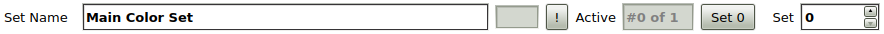
\includegraphics[scale=0.75]{main-window/main-window-bottom-1.png}
   \caption{Main Window Bottom, First Row}
   \label{fig:main_window_bottom_1}
\end{figure}

   \begin{itemize}
      \item \textbf{Set Name}
      \item \textbf{MG} (Mute Group)
      \item \textbf{Underrun Indicator}
      \item \textbf{Active Set Indicator}
      \item \textbf{Set Reset ("!")}
      \item \textbf{Set 0 Selector}
      \item \textbf{Set Changer}
   \end{itemize}

\subsubsection{Set Name}
\label{subsubsec:introduction_mg}

   This text field shows the name of the current set, and also allows editing
   the set name.
   The existing sets can be seen in the \textbf{Sets} tab.

\subsubsection{MG (Mute Group)}
\label{subsubsec:introduction_mute_group}

   This text field shows the name of the current mute-group, if one is
   in force. The existing mute-groups, if any, can be seen in the
   \textbf{Mutes} tab, or in the active 'mutes' files specified in the
   'rc' main configuration file.

\subsubsection{Underrun Indicator}
\label{subsubsec:introduction_underrun_indicator}

   This text field is empty under normal circumstances, including during
   playback.  However, if one opens a pattern editor for a pattern with a lot
   of events, and turns on recording for that pattern, then this field might
   start flashing numbers, which indicate the
   current underrun value in microseconds.  This gives an indication that
   timing of playback might be off a bit, usually less than 10 milliseconds.
   This happens because the event-list is locked during redrawing,
   when recording, to avoid problems when new notes come in.

\subsubsection{Active Set Indicator}
\label{subsubsec:introduction_active_set_indicator}

   This field shows the active set number, followed by the number of existing
   sets.
   Note that there is always at least one set in a \textsl{Seq66}
   tune.

\subsubsection{Set Reset ("!")}
\label{subsubsec:introduction_set_reset}

   This small button with an exclamation point
   to the right of the set name is meant to clear
   out all playing sets, and make only the current set the playing set.
   This button is useful when in "all-sets" mode or when sets get added
   automatically via the "additive" mode, so that multiple sets are playing
   at once.
   See \sectionref{subsec:configuration_rc}.

\subsubsection{Set Master Button}
\label{subsubsec:introduction_set_master_button}

   The Set Master button has been removed.
   The external window it used to bring up has been replaced
   by the \textbf{Set Master} tab.

%  This button brings up an external window showing the
%  panel.  This panel is also available in a center tab.  It is a work in
%  progress, and doesn't have a whole lot of functionality yet.
%  It can currently show existing sets in one view, and allow
%  reordering the sets.

\subsubsection{Active Set Indicator}
\label{subsubsec:introduction_active_set_indicator}

   This read-only text field shows the set number of the currently active set.
   One can open a number of external \textsl{Live Frames} by
   \textsl{shift-left-clicking} on pattern slots.
   The currently active set is then the
   set that has the mouse focus.  This allows for working with multiple sets
   without a lot of mouse/keyboard navigation.

\subsubsection{Set 0}
\label{subsubsec:introduction_set_zero}

   This button provides a fast way to get back to set 0, without clicking the
   mouse a bunch of times.
   It is useful when creating an external live grid
   (see \sectionref{fig:multiple_live_grids}),
   which currently also sets the main grid to the same set.
   Click on this button, and the external set and set 0 can be seen at the same
   time.

\subsubsection{Set Changer}
\label{subsubsec:introduction_set_changer}

   This spin-box allows showing a different set in the main windows.
   This set can be modified by adding new patterns, changing its name, or
   importing other MIDI files into the current set.

\subsection{Main Bottom Controls, Second Row}
\label{subsec:introduction_main_bottom_controls_2}

   Here is the second row and contents:

\begin{figure}[H]
   \centering 
   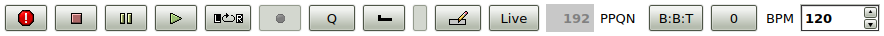
\includegraphics[scale=0.75]{main-window/main-window-bottom-2.png}
   \caption{Main Window Bottom, Second Row}
   \label{fig:main_window_bottom_2}
\end{figure}

   \begin{itemize}
      \item \textbf{Panic}
      \item \textbf{Stop}
      \item \textbf{Pause}
      \item \textbf{Play}
      \item \textbf{Record Button}
      \item \textbf{L/R Loop}
      \item \textbf{Live Song Record}
      \item \textbf{Keep Queue}
      \item \textbf{Mute Group Learn}
      \item \textbf{Developer Test}
      \item \textbf{Mute} (Toggle Mute Status)
      \item \textbf{Song Editor}
      \item \textbf{Live/Song}
      \item \textbf{PPQN Indicator}
      \item \textbf{Tap BPM}
      \item \textbf{Beats Per Minute Control}
   \end{itemize}

   Many of these controls have keystrokes and MIDI-control slots that can be
   set up in the 'ctrl' file.

   Note that \textbf{BBT/HMS Toggle Button} has been removed
   (version 0.99.9).
   One can now click on the \textbf{BBT/HMS Time Display} to
   change the format.

\subsubsection{Panic}
\label{subsubsec:introduction_panic_button}

   This button causes playback to stop, all patterns to mute, and flushes the
   MIDI buss.
   There is a keystroke control and a MIDI control
   for this automation operation, plus
   a MIDI-announcement (output) configuration item for it.

\subsubsection{Stop}
\label{subsubsec:introduction_stop_button}

   This button stops playback and rewinds to the beginning of the song.
   By default, the \texttt{Esc} key operates this function,
   and there is both a MIDI-control slot and a MIDI-announcement slot
   available for it.

\subsubsection{Pause}
\label{subsubsec:introduction_pause_button}

   This button stops playback, but does not rewind to the beginning of the
   song.  It also resumes playback at the same point as the pause.  By default,
   the \texttt{Period} key operates this function, and there is a MIDI-control
   slot and a MIDI-announcement slot available for it.  This key is also
   hardwired to pause and start playback in the pattern editor and the song
   editor.

\subsubsection{Play}
\label{subsubsec:introduction_play_button}

   This button starts playback, either at the beginning or at the pause point.
   Also called the "start button".
   By default, the \texttt{Space} key operates this function,
   and there is both a MIDI-control slot and a MIDI-announcement slot
   available for it.
   This key is also hardwired to toggle playback in the pattern editor and the
   song editor.

\subsubsection{Record Button}
\label{subsubsec:introduction_record_button}

   This button turns on recording for the various kinds of recording
   described in \sectionref{sec:recording}.
   Its color indicates the record-by feature in force:

   \begin{itemize}
      \item \textbf{Grey}.
         No pattern is selected, so this button is non-functional.
      \item \textbf{Red}.
         This color indicates the normal recording mode, which toggles only a
         single pattern for recording.
         This button is enabled and colored red only if a pattern is the last
         one selected in the grid.
      \item \textbf{Yellow}.
         This color indicates the record-by-channel recording mode,
         which toggles, for recording, all patterns that have an
         output channel set.
         Incoming events that have a channel nybble are routed to that
         pattern.
      \item \textbf{Green}.
         This color indicates the record-by-buss recording mode,
         which toggles, for recording, all patterns that have an
         input bus set. This button is green only if there is at least
         one such pattern.
         A pattern can be assigned an input buss via its right-click
         menu, but only if
         \textbf{Edit / Preferences / MIDI Input / Record into patterns by bus}
         is enabled.
   \end{itemize}

   These modes are selected in the 'rc' file as described in
   \sectionref{subsubsec:configuration_rc_midi_cmt}.
   They are mutually exclusive.

\subsubsection{L/R Loop}
\label{subsubsec:introduction_loop_button}

   This button has been added to the main window.
   It also appears in the "external" version of the song editor.
   This reflects that the \textbf{L/R} loop markers in the song editor can now
   be used in the pattern editor as well.  This new feature makes it easier to
   focus in on a pattern and tinker repeatedly with the same small section.
   In addition, looping can now be done in both the Live and Song modes of
   playback.

   \index{loop mode}
   Activates loop mode. When play is activated, plays the song and loop
   between the
   \index{L marker}
   \index{R marker}
   \textbf{L marker} and the \textbf{R marker}.
   It is a state button, and its appearance indicates when it is
   depressed, and thus active.
   \textsl{If this button is deactivated during playback, then playback
   continues past the \textbf{R marker}.}
   Note that these markers can be placed using left
   and right mouse clicks, respectively, in the time/measures ruler.
   Furthermore, the \textbf{L/R} markers can also be set in a pattern editor,
   where they can be used to focus in on a small section of notes.
   Lastly, this looping mechanism is also available in Live mode as well.

\subsubsection{Live Song Record}
\label{subsubsec:introduction_live_record_button}

   This button causes a live playing session to be recorded to Song mode.
   That is, triggers are added to the song automatically as the musician mutes
   and unmutes patterns, and the triggers can then be
   seen as layouts in the \textsl{Song} editor.
%  FIXME:
%  By default, the \texttt{P} key operates this function.

   Using the \texttt{Ctrl} modifier while clicking this button
   turns off the recording-snap feature.
   This change can also be done in the song editor.
   Using the \texttt{Shift} modifier while clicking this button
   causes recording immediately after starting playback.
   This feature is useful in avoid delay at start up.

\subsubsection{Keep Queue}
\label{subsubsec:introduction_keep_queue_button}

   Puts the application into a "sticky" queue mode.
   In this mode, pressing a pattern key does not do a mute/unmute function, but
   instead turns on queuing for the selected pattern.
   By default, the \texttt{Backslash} key operates this function,
   and there is a MIDI-control slot available for it.

\subsubsection{Mute Group Learn}
\label{subsubsec:introduction_mute_group_learn_button}

   \index{L button}
   Also called the "L" button.
   Sets up to learn the current set of active patterns ("mute group") into a
   mute-group.
   The default keystroke to control this button is lower-case "L".
   When in group-learn mode, the \texttt{Shift} key cannot be hit, so the
   group-learn mode automatically converts the keys to their shifted versions.
   This feature known as \textsl{shift-lock} or \textsl{auto-shift}.
   This feature is not used if a non-QWERTY keyboard layout is
   specified in the 'ctrl' file.

   After pressing the "L" button, the user can then press a keystroke, which is
   automatically shifted, and the pattern set is saved, and can be recalled by
   pressing that button, shifted, later.
   It can be saved in a 'mutes' file, as part of
   the MIDI tune, or in both places.

   \textsl{Example}:
   We have 5 patterns armed in the current set. Press the "L" button,
   and then press the "s" key.  These pattern statuses are saved and can be
   recalled later by the "S" ("s"-shifted) key.

   By default, the \texttt{el} (lower-case "L") key also sets this function,
   and there is a MIDI-control slot available for it, as well as a
   MIDI-announcement slot.
   In addition to that, one can also press
   the \texttt{Ctrl-L} key.
   The "el" with it!

   Remember that groups work with the playing ("in-view") screen-set.
   One must change the screenset and give it the command to make it the
   playing one.
   \index{keys!Home}
   By default, the \texttt{Home} key is configured for this purpose.

   There is also a setting in the 'mutes' file called
   \texttt{mute-group-selected}.  If this value is set to a value from 0 to 31,
   then that mute group will be automatically applied when
   \textsl{Seq66} starts up.
   This is useful with the loading of the most-recent MIDI file (which is also
   a feature of \textsl{Seq66}.
   Also see the section about the "mute master" tab,
   \sectionref{sec:mutes_master}.

\subsubsection{Developer Test}
\label{subsubsec:introduction_developer_test_button}

   This button is always disabled.  Functionality is added temporarily when
   testing new features. Ignore this button.

\subsubsection{Toggle Mute Status}
\label{subsubsec:introduction_toggle_mute_status_button}

   The \textbf{Mute}  button toggles the mute/armed status of all of the
   patterns in the current set.
   Works the same as the
   \textbf{Edit / Toggle All Tracks} menu or the hard-wired
   \texttt{Ctrl-T} key.
   There is also an automation control entry for it, associated by
   default with \texttt{F8}.
   As of version 0.99.16, it is no longer disabled in Song Mode.

\subsubsection{Song Editor}
\label{subsubsec:introduction_song_editor_button}

   This button (with a "pencil" icon)
   brings up an external window for editing the Song/Performance
   information.  If already up, it closes it.
   Works the same as the
   \textbf{Edit / Song Editor} menu or the hard-wired \texttt{Ctrl-E} key.

\subsubsection{Live/Song Mode}
\label{subsubsec:introduction_livesong_mode_button}

   This button toggles between the \textsl{Live} and \textsl{Song} performance
   mode. In the Live mode, the musician controls are muting/unmuting of each
   pattern.  In the Song mode, the triggers layed out in the
   \textbf{Song Editor} control the playback.
   By default, the \texttt{F10} key operates this function,
   There is also a MIDI automation control for this button.

\begin{comment}
   \itempar{Toggle Tracks}{pattern!toggle tracks}
   \index{pattern!toggle tracks}
   This button changes the status of all of the
   \textsl{playing} tracks, reversing the
   mute status of each pattern that is playing.
   The next click will then unmute only those tracks.
   Because it can be confusing, this button is disabled (not shown
   in the figure) in Song mode.

   The \texttt{Ctrl-M}, \texttt{Ctrl-U}, and \texttt{Ctrl-T} keys,
   as shown in the \textbf{Edit} menu, mute, unmute, and toggle
   all patterns.

\end{comment}

\subsubsection{PPQN Indicator}
\label{subsubsec:introduction_ppqn_indicator}

   This read-only field displays the current PPQN for the current tune.

   \configref{usr}{user-midi-settings}{midi\_ppqn}

\subsubsection{BBT/HMS Toggle (removed)}
\label{subsubsec:introduction_time_format_toggle_button}

   The time display has been converted to a button, and click it will
   switch the format. So the BBT/HMS Toggle button
   \textsl{has been removed}.
   See the top bar for the time display/button.

%  Toggles the format of the current time displayed during playback. 
%  It can be shown in B:B:T (bars:beats:ticks) or H:M:S (hours:minutes:seconds).

\subsubsection{Tap BPM Button}
\label{subsubsec:introduction_tap_bpm_button}

   Tap this button with a regular beat to determine the beats-per-minute of the
   tapping.  With each tap, the counter on the button increments and the BPM is
   recalculated.  Stop tapping for a few seconds to reset the counter.
   By default, the \texttt{F9} key operates this function, but it
   There is also a MIDI-control slot for this function, and
   \texttt{F9} is the default key for this function.

\subsubsection{Beats Per Minute Control}
\label{subsubsec:introduction_bpm_control}

   This control can be text-edited or spun to change the beats/minute value
   used in playing back the current song.  This value is also saved to the
   file.

%-------------------------------------------------------------------------------
% vim: ts=3 sw=3 et ft=tex
%-------------------------------------------------------------------------------
